%------------------------------------------------------------------------------
% CV in Latex
% Author : Huanfa Chen
% Inspired by and adapted from: https://github.com/sb2nov/resume and Jake's Resume on Overleaf
% Most recently updated version may be found at https://github.com/huanfachen/Huanfa_CV 
% License : MIT
%------------------------------------------------------------------------------

\documentclass[A4,11pt]{article}
% \usepackage[UTF8]{ctex}
%\documentclass[letterpaper,11pt]{article} %For use in US
% \usepackage{xeCJK}
% \usepackage{polyglossia}
\usepackage{CJKutf8}
\usepackage{latexsym}
\usepackage[empty]{fullpage}
\usepackage{titlesec}
\usepackage{marvosym}
\usepackage[usenames,dvipsnames]{color}
\usepackage{verbatim}
\usepackage{enumitem}
\usepackage[hidelinks]{hyperref}
\usepackage[english]{babel}
\usepackage{tabularx}
\usepackage{tikz}
% \usepackage{xeCJK}
% \usepackage{zh_CN-Adobefonts_external} 
% \setCJKmainfont{SimSun}
\input{glyphtounicode}

\begin{comment}
I am by no means a professional when it comes to the CV's/resumes, I have
received various trainings on how to write a CV and resume from my high 
school, as well as the Austin College and University of Eastern Finland's
career counseling departments. As I intend to share my CV as a template, I 
feel that it is my responsibility to provide explanations of my work.
\end{comment}

%% Set up citations and bibliography
\usepackage{bibunits}
\usepackage[sort&compress,super]{natbib}
\defaultbibliographystyle{apsrev4-2}
\setcitestyle{comma}
\setlength{\bibsep}{0pt}
\renewcommand{\bibnumfmt}[1]{\ \ \ #1.}
\renewcommand\refname{\vspace{-7mm}}
% \renewcommand\refname{}
\renewcommand{\bibsection}{}

%% This allows us to start a bibliography with arbitrary number
\usepackage{etoolbox}
\patchcmd{\thebibliography}{\section*{\refname}}{}{}{}
\makeatletter
\newcommand*{\newbibstartnumber}[1]{%
  \apptocmd{\thebibliography}{%
    \global\c@NAT@ctr #1\relax
    \addtocounter{NAT@ctr}{-1}%
  }{}{}%
}
\makeatother

%% Set up footer
\usepackage{fancyhdr}
\usepackage{lastpage}
\usepackage[nodayofweek,level]{datetime}
\fancypagestyle{CVfooter}
{
 \lhead{}
 \chead{}
 \rhead{}
 \lfoot{\small{Huanfa Chen}}
 \cfoot{\small{Last Update: \today}}
 \rfoot{\small{\thepage/\pageref{LastPage}}}
 \renewcommand{\headrulewidth}{0.0pt}
 \renewcommand{\footrulewidth}{0.5pt}
}

%-----FONT OPTIONS-------------------------------------------------------------
\begin{comment}
The font of the document will impact not just how readable it is, but how it is
perceived. In the "The Craft of Scientific Writing" by Michael Alley, shares a
common fonts for publication as well as their use. I have chosen to use
Palatino for its legibility, some others are given below. There is far too much
about typography to discus here. Note: serif fonts have short projecting
strokes, sans-serif fonts are sans (without) these strokes.
\end{comment}


% serif
 \usepackage{palatino}
% \usepackage{times} %This is the default as well
% \usepackage{charter}

% sans-serif
% \usepackage{helvet}
% \usepackage[sfdefault]{noto-sans}
% \usepackage[default]{sourcesanspro}

%-----PAGE SETUP---------------------------------------------------------------
% https://en.wikibooks.org/wiki/LaTeX/Page_Layout

% Adjust margins
% \usepackage[left=1.0in, right=1.0in, top=1.0in, bottom=1.0in]{geometry} % margins
% \usepackage{setspace}
% \singlespacing % No more than 6 lines of text per inch
\addtolength{\oddsidemargin}{-1cm}
\addtolength{\evensidemargin}{-1cm}
\addtolength{\textwidth}{2cm}
\addtolength{\topmargin}{-1cm}
\addtolength{\textheight}{2cm}
\addtolength{\footskip}{20pt}
% note the defatult footskip = 30 pt. Increasing the footskip will lower the position of the footer to the page bottom

% %% Page and text formatting
% \usepackage[left=1.0in, right=1.0in, top=1.0in, bottom=1.0in]{geometry} % margins
% \usepackage{setspace}
% \singlespacing % No more than 6 lines of text per inch
% \usepackage{amsmath, amsfonts}
% \usepackage[T1]{fontenc}
% \usepackage{times}

% Margins for US Letter size
%\addtolength{\oddsidemargin}{-0.5in}
%\addtolength{\evensidemargin}{-0.5in}
%\addtolength{\textwidth}{1in}
%\addtolength{\topmargin}{-.5in}
%\addtolength{\textheight}{1.0in}

\urlstyle{same}

\raggedbottom
\raggedright
\setlength{\tabcolsep}{0cm}

% Sections formatting
\titleformat{\section}{
  \vspace{-4pt}\scshape\raggedright\large
}{}{0em}{}[\color{black}\titlerule \vspace{-5pt}]

% Ensure that .pdf is machine readable/ATS parsable
\pdfgentounicode=1

%-----CUSTOM COMMANDS FOR FORMATTING SECTIONS----------------------------------
\newcommand{\CVItem}[1]{
  \item\small{
    {#1 \vspace{-2pt}}
  }
}

\newcommand{\MScStduentItem}[4]{
  \item #1 (#2, #3)
   \begin{itemize}
    \item[$\textendash$] \ #4
   \end{itemize}
}

\newcommand{\CVSubheading}[4]{
  \vspace{-2pt}\item
    \begin{tabular*}{0.97\textwidth}[t]{l@{\extracolsep{\fill}}r}
      \textbf{#1} & #2 \\
      \small#3 & \small #4 \\
    \end{tabular*}\vspace{-7pt}
}

\newcommand{\CVSubheadingSimple}[2]{
  \vspace{-2pt}\item
    \begin{tabular*}{0.97\textwidth}[t]{l@{\extracolsep{\fill}}r}
      \textbf{#1} & #2 \\
    \end{tabular*}\vspace{-7pt}
}

\newcommand{\CVSubSubheading}[2]{
    \item
    \begin{tabular*}{0.97\textwidth}{l@{\extracolsep{\fill}}r}
      \text{\small#1} & \text{\small #2} \\
    \end{tabular*}\vspace{-7pt}
}

\newcommand{\CVSubItem}[1]{\CVItem{#1}\vspace{-4pt}}

\renewcommand\labelitemii{$\vcenter{\hbox{\tiny$\bullet$}}$}

\newcommand{\CVSubHeadingListStart}{\begin{itemize}[leftmargin=0.5cm, label={}]}
% \newcommand{\resumeSubHeadingListStart}{\begin{itemize}[leftmargin=0.15in, label={}]} % Uncomment for US
\newcommand{\CVSubHeadingListEnd}{\end{itemize}}
\newcommand{\CVItemListStart}{\begin{itemize}}
\newcommand{\CVItemListEnd}{\end{itemize}\vspace{-5pt}}

%------------------------------------------------------------------------------
% CV STARTS HERE  %
%------------------------------------------------------------------------------
\begin{document}
\begin{CJK*}{UTF8}{gbsn}
\pagestyle{CVfooter}

%-----HEADING------------------------------------------------------------------
\begin{comment}
Avoid using photos in academic CV
\end{comment}

\begin{minipage}[c]{0.05\textwidth}
\-\
\end{minipage}
\begin{minipage}[c]{0.2\textwidth}
\begin{tikzpicture}
    % \clip (0,0) circle (1.75cm);
    \node at (0,-.7) {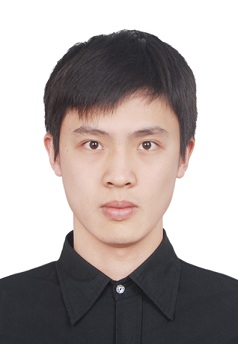
\includegraphics[width = 3cm]{Photo_Huanfa_Chen.jpg}}; 
    % if necessary the picture may be moved by changing the at (coordinates)
    % width defines the 'zoom' of the picture
\end{tikzpicture}
\hfill\vline\hfill
\end{minipage}
\begin{minipage}[c]{0.05\textwidth}
\-\
\end{minipage}
% \hfill
\begin{minipage}[c]{0.4\textwidth}
    \textbf{\Huge \scshape 陈焕发} \\ \vspace{1pt}
    
    % \textbf{陈焕发} \\ \vspace{1pt}
    % \scshape sets small capital letters, remove if desired
    \small{电话:+44 7737106369} \\
    \small{微信:huanfa\_forever} \\
    \href{mailto:chenhuanfa@gmail.com}{\underline{chenhuanfa@gmail.com}}\\
    % Be sure to use a professional *personal* email address
    \href{https://www.linkedin.com/in/huanfa-chen/}{\underline{linkedin.com/in/huanfa-chen}} \\
    % you should adjust you linked in profile name to be professional and recognizable
    \href{https://github.com/huanfachen}{\underline{github.com/huanfachen}}
\end{minipage}

% Without picture
% \begin{center}
%     \textbf{\Huge \scshape Huanfa Chen} \\ \vspace{1pt} %\scshape sets small capital letters, remove if desired
%     % \small +1 123-456-7890 $|$ 
%     \href{mailto:huanfa.chen@ucl.ac.uk}{\underline{huanfa.chen@ucl.ac.uk}} $|$
%     \href{huanfachen.github.io}{\underline{https://huanfachen.github.io/}} $|$\\
%     % Be sure to use a professional *personal* email address
%     \href{linkedin.com/in/huanfa-chen}{\underline{linkedin.com/in/huanfa-chen}} $|$
%     % you should adjust you linked in profile name to be professional and recognizable
%     \href{https://github.com/huanfachen}{\underline{github.com/huanfachen}}
% \end{center}

\begin{comment}
This CV was written for specifically for positions I was applying for in
academia, and then modified to be a template.

A standard CV is about two pages long where as a resume in the US is one page.
sections can be added and removed here with this in mind. In my experience, 
education, and applicable work experience and skills are the most import things
to include on a resume. For a CV the Europass CV suggests the categories: Work
Experience, Education and Training, Language Skills, Digital Skills,
Communication and Interpersonal Skills, Conferences and Seminars, Creative Works
Driver's License, Hobbies and Interests, Honors and Awards, Management and
Leadership Skills, Networks and Memberships, Organizational Skills, Projects,
Publications, Recommendations, Social and Political Activities, Volunteering.

Your goal is to convey a who, what , when, where, why for every item you share. 
The who is obviously you, but I believe the rest should be done in that order.
For example below. An employer cares most about the degree held and typically 
less about the institution or where it is located (This is still good 
information though). Whatever order you choose be consistent throughout.
\end{comment}

%-----EDUCATION----------------------------------------------------------------
\section{教育经历}
  \CVSubHeadingListStart
%    \CVSubheading % Example
%      {Degree Achieved}{Years of Study}
%      {Institution of Study}{Where it is located}
    \CVSubheading
      {{\textbf{理学博士}  $,$ \emph{\small{地理信息科学}}}}{2014 -- 2019}
      {伦敦大学学院(UCL)(导师:Tao Cheng教授)}{英国}
    \CVSubheading
      {{理学硕士  $,$ \emph{\small{地图学与地理信息系统}}}}{2011 -- 2014}
      {北京大学(导师:李琦教授)}{中国}
    \CVSubheading
      {{理学学士  $,$ \emph{\small{化学}}}}{2007 -- 2011}
      {北京大学}{中国}
  \CVSubHeadingListEnd

%-----WORK EXPERIENCE----------------------------------------------------------
\begin{comment}
try to briefly explain what you did and why it is relevant to the position you
are seeking
\end{comment}

\section{工作经历}
  \CVSubHeadingListStart
%    \CVSubheading %Example
%      {What you did}{When you worked there}
%      {Who you worked for}{Where they are located}
%      \CVItemListStart
%        \CVItem{Why it is important to this employer}
%      \CVItemListEnd
    \CVSubheading
      {\textbf{讲师(助理教授)},空间数据科学方向}{2020年10月 --}
      {高级空间分析中心, UCL}{英国}
      \CVItemListStart
        \CVItem{博士生导师;讲授研究生课程}        
        \CVItem{副系教务主任 (2020年起)}
      \CVItemListEnd
    \CVSubheading
    {教员,空间数据科学方向}{2019年2月 -- 2020年10月}
      {高级空间分析中心, UCL}{英国}
      \CVItemListStart
        \CVItem{博士生导师;讲授研究生课程}        
        \CVItem{副系教务主任 (2020年起)}
      \CVItemListEnd
    \CVSubheading
      {客座教授}{2019年1月 --}
      {建筑与城市学院, University of Westminster}{英国}
      \CVItemListStart
        \CVItem{讲授GIS和空间分析课程}
    \CVItemListEnd
    \CVSubheading
      {助教}{2014年10月 -- 2019年1月}
      {土木环境与测绘系,UCL}{英国}
      \CVItemListStart
        \CVItem{讲授“多智能体仿真”硕士生课程}
        \CVItem{主持R/Python/NetLogo习题课}
      \CVItemListEnd
     \CVSubheading
      {研究助理}{2015年10月 -- 2019年1月}
      {土木环境与测绘系,UCL}{英国}
      \CVItemListStart
        \CVItem{参与"犯罪,警务与市民信心"科研项目,受英国物理与工程科学基金委(EPSRC)资助}
        \CVItem{开发时空犯罪热点预测算法和可视化系统}
      \CVItemListEnd
  \CVSubHeadingListEnd

%-----RESEARCH INTERESTS----------------------------------------------------------
\begin{comment}
try to briefly explain what you did and why it is relevant to the position you
are seeking
\end{comment}

\section{研究兴趣}
  \CVSubHeadingListStart
%    \CVSubheading %Example
%      {What you did}{When you worked there}
%      {Who you worked for}{Where they are located}
%      \CVItemListStart
%        \CVItem{Why it is important to this employer}
%      \CVItemListEnd
    \CVSubheading
      {空间优化}{}
      {选址,路径规划,区划等问题的模型开发,应用于城市管理/犯罪预防/警员巡逻}{}
    \CVSubheading
      {时空人工智能}{}
      {基于时空大数据的人工智能模型研发,并应用于预测犯罪热点,交通流量等}{}
    \CVSubheading
      {城市居民移动模式}{}
      {融合经济计量学和机器学习模型,预测和理解居民的出行交通模式和目的}{}
    \CVSubheading
      {健康GIS}{}
      {应用GIS方法以理解传染病的时空模式,并制定防控措施}{}

    
  \CVSubHeadingListEnd

%-----Publications----------------------------------------------------------
\section{研究成果}

\vspace{2mm}
\noindent \textbf{\ \ \underline{期刊论文}}
\begin{bibunit}
\nocite{apsrev42Control}
\nocite{Chen2021, Chen2019ijgis, Chen2018ijgis, Chen2017CEUS, Aslam2021, Ren2020ijgis, Zhang2021cities, Qiao2011langmuir, Qiao2011jpcc, Qiao2010jpcb}
\putbib[publications]
\end{bibunit}

\vspace{2mm}
\noindent \textbf{\ \ \underline{书籍章节}}
\begin{bibunit}
\nocite{apsrev42Control}
\nocite{Chen2021chapter}
\putbib[publications]
\end{bibunit}

\vspace{2mm}
\noindent \textbf{\ \ \underline{正在评审论文}}
\begin{bibunit}
\nocite{apsrev42Control}
\nocite{Huanfa2021trans, Huanfa2022IEEEITS, Huanfa2022AAAG, Huanfa2022EPB, Yutong2022TBS, Bei2022GSIS, Hongbiao2022AE}
\putbib[publications]
\end{bibunit}

\vspace{2mm}
\noindent \textbf{\ \ \underline{会议论文}}
\begin{bibunit}
\nocite{apsrev42Control}
\nocite{Huanfa2020gisruk,Huanfa2019gisruk,Huanfa2017gisruk,Huanfa2017geocomp,Yajie2013geocomp,Huanfa2013ICESEP,Hamed2013ICESEP}
\putbib[publications]
\end{bibunit}

\vspace{2mm}
\noindent \textbf{\ \ \underline{项目报告}}
\begin{bibunit}
\nocite{apsrev42Control}
\nocite{Cheng2016cpc}
\putbib[publications]
\end{bibunit}

\vspace{2mm}
\noindent \textbf{\ \ \underline{软件项目}}
\begin{bibunit}
% \nocite{apsrev42Control}
\nocite{}
\putbib[publications]
\end{bibunit}

\vspace{2mm}
\noindent \textbf{\ \ \underline{其他研究成果}}
\newbibstartnumber{6}
\begin{bibunit}
\nocite{apsrev42Control}
% \nocite{CominScience2014,ZeljkovicNanoLetters2014,SoumyanarayananPNAS2013,ZeljkovicScience2012,HoffmanScience2002qpi}
\putbib[publications]
\end{bibunit}

%-----PROJECTS AND RESEARCH----------------------------------------------------
\begin{comment}
\end{comment}

\section{指导学生}
\vspace{2mm}
\begin{enumerate}
   \item 伦敦大学学院, 英国, 2019 --
     \begin{enumerate}
       \item \underline{博士生 (作为第二导师)}
       \begin{enumerate}
           \item Xiaowei Gao (PhD Geographical Information Science, 2020 --)
           \begin{itemize}
            \item[$\textendash$] \ Research area: Spatio-temporal analytics of cycling mobility
           \end{itemize}
           \item Meihui Wang (PhD Geographical Information Science, 2020 --)
           \begin{itemize}
            \item[$\textendash$] \ Research area: Urban analytics based on street-view imagery
           \end{itemize}
       \end{enumerate}
       \item \underline{硕士生 (共指导30名硕士生,以下是部分学生的论文题目)}
       \begin{enumerate}
           \MScStduentItem{Lingru Feng}{MSc Spatial Data Science and Visualisation}{2020 -- 2021}
           {Thesis: Comparing Floating Catchment Area Methods for Measuring Spatial Accessibility to COVID-19 Vaccination Service in England}
           \MScStduentItem{Chenxi Zhao}{MSc Spatial Data Science and Visualisation}{2020 -- 2021}
           {Thesis: The relationship between covid-19 and socio-demographic in London: the three lockdowns in 2020}
           \MScStduentItem{Huaming Yan}{MSc Spatial Data Science and Visualisation}{2020 -- 2021}
           {Thesis: Using spatial analysis to measure the fire incidents response time in Greater London}
           \MScStduentItem{Yutong Xia}{MSc Smart Cities and Urban Analytics}{2020 -- 2021}
           {Thesis: A Random Effect Bayesian Neural Network (RE-BNN) for Choice Analysis: Predicting Travel Mode Choice Across Multiple Regions}
           \MScStduentItem{Yixin Huang}{MSc Smart Cities and Urban Analytics}{2020 -- 2021}
           {Thesis: Research on spatial accessibility and spatial inequality of vaccination sites in England}
           \MScStduentItem{Xiaohan Feng}{MSc Spatial Data Science and Visualisation}{2020 -- 2021}
           {Thesis: Decomposition Analysis of Index of Multiple Deprivation (IMD) Based on Shapley Value}
           \MScStduentItem{Xiaomei Ge}{MSc Smart Cities and Urban Analytics}{2019 -- 2020}
           {Thesis: Looking into home sharing platforms and their influence on local inequality and insecurity: a case study of London}
           \MScStduentItem{Chuyin Deng} {MSc Spatial Data Science and Visualisation}{2019 -- 2020}
            {Thesis: Exploring the influential factors of cases growth of COVID-19 with machine learning techniques}
           \MScStduentItem{Zhenzhi Zhang}{MSc Spatial Data Science and Visualisation}{2019 -- 2020}
            {Thesis: Understanding public confidence towards NHS by ordered logistics regression based on survey results}
          \MScStduentItem{Xiang Zhou}{MSc Spatial Data Science and Visualisation}{2019 -- 2020}
           {Thesis: Solving vehicle routing problems in supply chain using genetic algorithms: a case study in Shanghai}
          \MScStduentItem{Yu Fu}{MSc Spatial Data Science and Visualisation}{2019 -- 2020}
           {Thesis: A real-time forecast of electricity consumption in residential buildings using machine learning approaches}
          \MScStduentItem{Thomas Keel}{MSc Spatial Data Science and Visualisation}{2018 -- 2019}
           {Thesis: Can we predict why people travel within a city? A cast study in Montreal, Canada}
          \MScStduentItem{Yang Zhou}{MSc Smart Cities and Urban Analytics}{2018 -- 2019}
           {Thesis: Retail centre footfall: planning and forecasting using time series modelling}
          \MScStduentItem{Yafei Ye}{MRes Spatial Data Science and Visualisation}{2018 -- 2019}
           {Thesis: Understanding residents’ attitudes towards services and safety issues by geodemographics based on city survey results}
          \MScStduentItem{Yunong Wang}{MSc Spatial Data Science and Visualisation}{2018 -- 2019}
           {Thesis: Optimal siting and sizing of electric vehicle charging points: a case study in London}
          \MScStduentItem{Maria del pilar Mayora}{MSc Smart Cities and Urban Analytics}{2018 -- 2019}
           {Thesis: An environmental bicycle level of service index for the Buenos Aires cycle network}
          \MScStduentItem{Ziyi Cheng}{MSc Smart Cities and Urban Analytics}{2018 -- 2019}
           {Thesis: Exploring the spatial accessibility to green space in the Greater London area}

% If you want to add a new student, use the following template
        % \MScStduentItem{STUDENT_NAME}{MSc_PROGRAMME}{2019 -- 2020}
        %   {Thesis: Exploring the Spatial Accessibility to Green Space in the Greater London Area}
       \end{enumerate}
     \end{enumerate}
\end{enumerate}  

%-----PROJECTS AND RESEARCH----------------------------------------------------
\begin{comment}
Ideally the title of the work should speak for what it is. However if you feel
like you should explain more about why the project is applicable to this job,
use item list as is shown in the work experience section.
\end{comment}

% \section{Projects and Research}
%   \CVSubHeadingListStart
% %    \CVSubheading
% %      {Title of Work}{When it was done}
% %      {Institution you worked with}{unused}
%     \CVSubheading
%       {{Surface Plasmon Propagation in the Kretschmann-Raether Configuration} $|$ \emph{\small{Python}}}{Fall 2020}
%       {University of Eastern Finland}{}
%     \CVSubheading
%       {{Simulation of Vector Beams Through High Numerical Aperture Lens} $|$ \emph{\small{Python}}}{Fall 2020}
%       {University of Eastern Finland}{}
%     \CVSubheading
%       {Characterization of the Flame-S Spectrometer for Spectral Imaging Research}{Spring 2020}
%       {University of Eastern Finland}{}
%     \CVSubheading
%       {{Free Form Lens Systems for 3D Printing} $|$ \emph{\small{MATLAB, OpTaliX}}}{Spring 2019}
%       {University of Eastern Finland}{}
%     \CVSubheading
%       {Procedures for Plating and Wet-Etching in III-V Semiconductor Devices}{Summer 2019}
%       {Finisar Corp.}{}
%     \CVSubheading
%       {Photo-Filter Characterization for Photometric Identification of Be Stars}{Fall 2017}
%       {Austin College}{}
%     \CVSubheading
%       {Improved Calibrating Equations for Volumetric Soil Moisture Measurement}{Spring 2017}
%       {Austin College}{}
%     \CVSubheading
%       {{Product Design, and Manufacturing Using 3D Printing} $|$ \emph{\small{Autodesk 123D}}}{Fall 2016}
%       {Austin College}{}
%   \CVSubHeadingListEnd

%-----CONFERENCES AND PRESENTATIONS--------------------------------------------
\begin{comment}
Again the title should have already been enough, but if it is necessary to add
descriptions maintain the consistency from prior sections
\end{comment}

\section{会议报告}
\noindent \textbf{\ \ \underline{受邀报告}}
  \CVSubHeadingListStart
%    \CVSubheading % Example
%      {Work Presented}{When}
%      {Occasion}{}
    \CVSubheading
      {Geospatial machine learning: motivations and implications}{2020年5月}
      {天津大学建筑学院}{}
    \CVSubheading
      {Machine learning for urban analytics and transport studies}{2021年3月}
      {中国测绘科学研究院}{}
    % \CVSubheading
    %   {Design and Manufacturing of Products using 3D Printing}{April 2017}
    %   {Austin College Student Scholarship Conference}{}
  \CVSubHeadingListEnd

%-----HONORS AND AWARDS--------------------------------------------------------
\section{荣誉和奖励}
  \CVSubHeadingListStart
%    \CVSubheading %Example
%      {What}{When}
%      {Short Description}{}
    \CVSubheading
      {UCL Q-Step学生实习项目}{2021}
      {\textsterling 3,000 资助,指导本科生科研项目}{UCL, 英国}
      \CVItemListStart
        \CVItem{科研项目:评估全球多国家的Covid-19疫苗服务的可达性}
      \CVItemListEnd
    % \CVSubheading
    \CVSubheading
      {2019 AAG Applied Geography Specialty Group Project Development Award}{2019}
      {\$500 资助,支持“预测城市地区共享单车需求”的研究项目}{美国}
    \CVSubheading
      {2019 AAG Applied Geography Specialty Group Travel Award}{2019}
      {\$250 参会补贴}{US}
    \CVSubheading
      {Roger Tomlinson论文奖}{2018}
      {由ESRI公司资助,授予UCL指导的地理信息科学方向最佳博士论文}{UCL, 英国}
    \CVSubheading
      {EPSRC互联社会先行者比赛决赛选手}{2018}
      {由英国物理与工程科学基金会发起的比赛,全英国共500名多领域的博士生参赛,决赛名单共16人}{英国}
    \CVSubheading
      {上海开放数据应用大赛“明日之星”奖励}{2017}
      {领队,负责项目管理和算法开发}{上海,中国}
      \CVItemListStart
        \CVItem{项目内容:共享单车的站点选址和运营优化}
      \CVItemListEnd
    \CVSubheading
      {年轻研究者的旅行补贴}{2017}
      {获得 €300 资助,以参加研讨会}{Leiden University, 荷兰}
      \CVItemListStart
        \CVItem{研讨会主题:"移动模式:新传感器,新数据,新挑战"}
      \CVItemListEnd
    \CVSubheading
      {UCL-CSC 联合博士奖学金}{2014 -- 2018}
      {博士全额奖学金,资助期限四年}{UCL, 英国}
    \CVSubheading
      {2015年ISPRS开发数据全球挑战赛优秀奖}{2015}
      {作为队长,带队在初赛排名前十(共100个队伍参赛)}{深圳大学, 中国}
    \CVSubheading
      {最佳青年学者论文提名奖}{2015}
      {在首届时空计算国际会议获得 \$500 奖励}{乔治梅森大学, 美国}
    \CVSubheading
      {北京大学-中石油奖学金}{2010}
      {学业成绩在全年级排名前10/150;奖金 \textyen5,000}{北京大学, 中国}
    \CVSubheading
      {北京大学三好学生}{2008}
      {学业成绩在全年级排名前20/150}{北京大学, China}
      
  \CVSubHeadingListEnd

%-----TEACHING EXPERIENCE------------------------------------------------------
\begin{comment}
Section is here as it applied to my application for positions in academia. 
Remember to tailor the resume for to the position.
\end{comment}

\section{教学经历}
  \CVSubHeadingListStart
%    \CVSubheading
%      {What}{When}
%      {School}{Where}
    \CVSubheading
      {CASA0007: 定量方法}{2019 --}
      {教授城市研究和空间分析的数学方法基础}{UCL}
    \CVSubheading
      {CASA0013: 空间数据科学基础}{2019 --}
      {基于Python的空间数据科学, 涵盖pandas/geopandas/matplotlib/sklearn}{UCL}
    \CVSubheading
      {CASA0006: 空间数据科学}{2019 --}
      {基于统计学习和机器学习的空间分析方法}{UCL}
    \CVSubheading
      {CASA0009: 空间数据获取,存储与分析}{2019 --}
      {涵盖MySQL数据库, Javascript, WebGIS网站建设}{UCL}
    \CVSubheading
      {CASA0011: 空间多智能体模型}{2021 --}
      {基于NetLogo编程的空间显式多智能体模型}{UCL}
    \CVSubheading
      {CEGE0076: 时空数据挖掘}{2015 -- 2021}
      {基于R语言,介绍时空数据挖掘常用模型和方法}{UCL}
    \CVSubheading
      {CEGE0082: GIS思想与方法}{2016 -- 2017}
      {讲授基于ArcGIS的GIS习题课}{UCL}
  \CVSubHeadingListEnd

%-----COMMUNITY INVOLVEMENT----------------------------------------------------
\section{协会活动}
\noindent \textbf{\ \ \underline{协会会员}}
  \CVSubHeadingListStart
%    \CVSubheading %Example
%      {What you did}{When you worked there}
%      {Who you worked for}{Where they are located}
    \CVSubheading
      {会员, 美国地理学家协会}{2015 -- }
      {}{}
  \CVSubHeadingListEnd

\noindent \textbf{\ \ \underline{协会任职}}
  \CVSubHeadingListStart
%    \CVSubheading %Example
%      {What you did}{When you worked there}
%      {Who you worked for}{Where they are located}
    \CVSubheading
      {理事会成员, 国际华人地理信息科学协会}{2021 -- }
      {}{}
    \CVSubheading
      {秘书长,北京大学全英校友会}{2016 -- 2018}
      {主持20人的理事会,组织150名参会人员的年会}{英国}
    %   {Oversaw a 10\% membership boost compared to the previous year}
    \CVSubheading
      {主席, 伦敦博士联盟}{2016 --}
      {组织多学科领域的学术研讨会;协会共有800名成员}{英国}
  \CVSubHeadingListEnd

\section{期刊编辑}
  \CVSubHeadingListStart
    \CVSubheadingSimple
      {编委会成员, Humanities and Social Sciences Communications}{2022 --}
      
    \CVSubheading
      {客座编辑,负责Covid-19 Impact on Human Mobility特刊}{2021 -- 2022}
      {Geo-spatial Information Science}{}
      
  \CVSubHeadingListEnd

\section{评审经历}
\noindent \textbf{\ \ \underline{期刊审稿}}
  \CVSubHeadingListStart

    \CVSubheadingSimple
      {International Journal of Geographic Information Science}{2015 --}
    \CVSubheadingSimple
      {Computers, Environments, and Urban Systems}{2018 --}
    \CVSubheadingSimple
      {Transportation Research Part C: Emerging Technologies}{2019 --}
    \CVSubheadingSimple
      {Journal of Homeland Security and Emergency Management}{2022 --}
  \CVSubHeadingListEnd




%-----SKILLS-------------------------------------------------------------------
\begin{comment}
This section is compressed from the various skills sections that Euro CV
recommends.
\end{comment}

\section{技能}
 \begin{itemize}[leftmargin=0.5cm, label={}]
    \small{\item{
     \textbf{语言}{: 普通话, 英语, 粤语,潮汕话} \\
     \textbf{编程}{: Python, R, Java, C++, Linux Bash} \\
     \textbf{软件系统}{: Esri ArcGIS, Microsoft Office Suite, LaTex, Markdown} \\
     \textbf{业余兴趣}{: 羽毛球, 旅行, 阅读, 博客写作} \\
    }}
 \end{itemize}
    
%------------------------------------------------------------------------------
\end{CJK*}
\end{document}